%!TEX root = ../thesis.tex

% Definitions:
%%%%%%%%%%%%%%
% Semantiv Web = samantisches Web

\chapter{Grundlagen} % (fold)
\label{cha:grundlagen}

\todo[inline]{\Huge mehr QUELLEN!!!}

\section{Zugriff auf Webanwendungen} % (fold)
\label{sec:zugriff_auf_webanwendungen}

Der Zugriff auf Daten von einer Webanwendung ist in den seltensten Fällen durch eine direkte Anbindung an die dahinter liegende Datenbank möglich beziehungsweise gewünscht. Gerade wenn das eigene Geschäft von diesen Daten abhängt, will man nur ungern alles mit allen teilen. Um trotzdem Dritten die Nutzung zu ermöglichen, wird dazu eine eine der Zugriff über eine vordefinierte Schnittstelle gestattet. Für Anwendungen und Dienste im Web sind die folgenden zwei Ansätze für die Architektur einer solchen Schnittstellen besonders verbreitet. 

\subsection{Representational State Transfer (REST)} % (fold)
\label{sub:rest}

Eine sehr beliebte Architektur für den öffentlichen Zugriff auf Webanwendungen ist \emph{Representational State Transfer} (REST) \cite[S.\,76]{fielding2000architectural}. REST baut auf HTTP auf und definiert einige Beschränkungen die eine REST basierter Dienst erfüllen muss. 

\medskip

Die Grundidee besteht darin, dass hinter einer URL eine bestimmte Ressource sich verbirgt auf die man von außen zugreifen möchte. REST schreib aber nicht vor in welchen Datenformat diese Ressource übermittelt werden soll, sondern dass das zurückgelieferte Format der Ressource änderbar ist. 


\begin{quote}
\enquote{REST components communicate by transferring a representation of a resource
in a format matching one of an evolving set of standard data types, selected dynamically
based on the capabilities or desires of the recipient and the nature of the resource.}\cite[S.\,87]{fielding2000architectural} 

\end{quote}

Dadurch soll einer einfachere Verwendbarkeit in unterschiedliche Systemen ermöglicht werden. So kann für eine Webanwendung beim aufrufen im Browser eine HTML-Datei zurück geliefert werden, die sofort betrachtet werden kann und falls ein Programm darauf zugreift wird ein maschinenlesbares Format verwendet. Neben HTML sind auch noch XML und JSON sehr verbreitete Formate. Die Kommunikation wird dabei komplett Zustandslos abgehalten und alle Zusatzinformationen müssen immer mitgeliefert werden. Durch die Zustandslosigkeit skaliert das System viel besser, da Ressourcen sofort wieder frei gegeben werden können und nicht für spätere Anfragen gespeichert werden müssen. 


\begin{table}[ht]
\centering
\caption{Wichtigsten HTTP Operationen mit REST} 
\begin{tabular}{r|p{12cm}}
    \textbf{Operation} & 
    \textbf{Beschreibung} \\ 
    \hline
    \texttt{GET} & 
    Liefert die hinter einer URL liegende Ressource an den Aufrufer zurück.\\
    
    \texttt{POST} & 
    Dient zum Anlegen einer neuen Ressource. Die URI der neuen Ressource ist beim Aufruf noch unbekannt und wird von Service bestimmt. \\

    \texttt{PUT} & 
    Wird zum Ändern eine bestehenden Ressource genutzt. \\
    
    \texttt{DELETE} &
    löscht, wie der Name schon sagt, eine Ressource dauerhaft.
\end{tabular}
\label{tbl:rest_oprations}
\end{table} 

\medskip

Wie schon beschrieben, nutzen REST basierte Dienste HTTP als Grundlage zur Kommunikation. Die dort definierten Operationen werden mit REST zur Auslieferung und Manipulation der Ressourcen verwendet. Zur Grundausstattung  gehören dabei \texttt{GET}, \texttt{POST}, \texttt{PUT} und \texttt{DELETE} (siehe Tabelle \ref{tbl:rest_oprations}). Die anderen Operationen \texttt{HEAD}, \texttt{TRACE}, \texttt{OPTIONS} und \texttt{CONNECT} sind eher selten anzutreffen.
     
% subsection rest (end)

\subsection{Simple Object Access Protocol (SOAP)} % (fold)
\label{sub:soap}

Das \emph{Simple Object Access Protocol}\cite{Mitra2007} (SOAP) ist ein vom W3C standardisiertes Netzwerkprotokoll für den Austausch von Daten zwischen heterogenen Systemen. SOAP schreibt einen bestimmten Aufbau von Nachrichten vor, innerhalb von denen die Daten transportiert werden. Als Repräsentation für diese Nachrichten wird auf XML gesetzt. Bei der Wahl des Transportprotokolls werden dahingegen keine Vorgaben gemacht und es ist frei wählbar. Häufig wird es aber in Verbindung mit HTTP und TCP verwendet. 

\medskip

\begin{lstlisting}[
    language=XML,
    caption={SOAP Nachricht}\label{lst:soap_nachricht},
    captionpos=t]
<Envelope xmlns="http://www.w3.org/2003/05/soap-envelope">
    <Header>
        <!-- header information -->
    <Header> 
    <Body>
        <!--body content-->
    </Body>
</Envelope>
\end{lstlisting}

Eine Nachricht besteht im Grunde aus drei Elementen: den \emph{Envelope}, einen optionalen \emph{Header} und einem \emph{Body} (siehe Listing \ref{lst:soap_nachricht}). Der Envelope fungiert, wie die Übersetzung schon sagt, als Briefumschlag für die zu transportierenden Daten. Innerhalb jedes Envelopes können zusätzliche Meta-Informationen im Header Element gespeichert werden. Die eigentlichen Daten befinden sich im Body Element des Evelopes. Wie der Inhalt von Header und Body auszusehen haben wird von SOAP nicht vorgeschrieben. Dies können weitere XML Elemente oder einfache Zeichenketten sein. 

\subsubsection{Web Services Description Language} % (fold)
\label{ssub:wsdl}

% subsubsection wsdl (end)

Gebräuchlich ist der Einsatz von SOAP bei sogenannten \emph{Remote Procedure  Calls} (RPC). Unter RPC verseht man den Aufruf eine Funktion von einem entfernten Dienst und das Zurückliefern einer eventuell vorhandenen Antwort. Welche Funktionen von einen Dienst zur Verfügung stehen wird ein einer \emph{Web Services Description Language}\cite{wsdl2001} (WSDL) Datei beschrieben. Diese WSDL Datei wird in XML Format geschrieben und enthält alle wichtigen Informationen für RPC Aufrufe, die von einen Dienst zur Verfügung gestellt werden: 

\begin{description}
    \item[\textbf{types}] enthält Definition von Datentypen die in einer Message eingesetzt werden können. Zur Definition der Datentypen wird das Vokabular von XML Schema\footnote{\url{http://www.w3.org/XML/Schema}} eingesetzt.
    \item[\textbf{message}] Elemente beschreiben die Datentypen aus denen eine Nachricht aufgebaut ist.
    \item[\textbf{portType}] definiert eine Menge an zur Verfügung stehenden Operationen. Inklusive Eingabe- und Ausgabeparameter. In der WSDL Version 2.0 wurde portType in \emph{interface} umbenannt.
    \item[\textbf{binding}] beschreibt das Format und den Protokollablauf mehrerer Operationen. Zum Beispiel wie Eingabe- und Ausgabeparameter kodiert werden sollen. 
    \item[\textbf{port}] Definiert eine Adresse hinter der sich ein Binding befindet. Üblicherweise in Form ein URI. Seit WSDL 2.0 wird statt port der Begriff \emph{endpoint} verwendet.
    \item[\textbf{service}] dient zum Zusammenfassen mehrerer Ports zu einen einzigen Dienst.
\end{description}

Wird eine solche WSDL Datei öffentlich zugänglich gemacht, kann festgestellt werden welche Funktionen ein Dienst anbietet und automatisch Schnittstellen für unterschiedliche Systeme generiert werden. Der weiter Datenaustausch erfolgt dann über SOAP Nachrichten.

% subsection wsdl_und_soap (end)


% section zugriff_auf_webanwendungen (end)

\section{Datenintegration} % (fold)
\label{sec:datenintegration}

% section datenintegration (end)


\subsection{Semantic web und das Resource Description Framework} % (fold)
\label{sub:semantic_web_und_das_resource_description_framework}



\todo[inline]{Idee semantic web einbauen}

Eine der bekanntesten Umsetzungen der Vision des  semantischen Webs ist wohl das \emph{Resource Description Framework} (RDF). Wie der Name schon suggeriert dient RDF zur Beschreibung von einzelnen Ressourcen innerhalb des Internets. Nach \cite{Klyne2004,Manola2004} bestand die Motivation bei der Entwicklung von RDF Information über Ressource in einen offenen Datenmodell zu speichern, so dass diese Daten von Maschinen automatisch verarbeitet, manipulieren und untereinander ausgetauscht werden können. Gleichzeitig sollte es auch einfach von jedem erweitert werden können \enquote{RDF is designed to represent information in a minimally constraining, flexible way}\cite{Klyne2004}.

\medskip

Das Datenmodell von RDF ist zur effizienten Verarbeitung sehr einfach aufgebaut. Die Grundlage bilden Tripel aus Subjekt, Prädikat und Objekt. Einer oder mehrere solcher Triple zusammen werden als gerichteter RDF-Graph bezeichnet. Subjekt und Objekt stehen über das Prädikat mit einander in Beziehung, wobei die Beziehung immer vom Subjekt zum Objekt geht. Das Prädikat wird auch als Eigenschaft (engl. Property) bezeichnet. Gemeinsam beschreibt das Triple immer eine Aussage über eine oder zwei Ressourcen. Zum Beispiel \enquote{Die Dose enthält Kekse} wäre eine Aussage, dass in einer Dose sich Kekse befinden. Die Dose ist dabei das Subjekt, enthält das Prädikat und Kekse das Objekt. Ein Triple ist quasi ein einfacher Satz in der natürlichen Sprache \cite{Heinzen}. Für Subjekt, Prädikat und Objekt werden in RDF \emph{Uniform Resource Identifier} (URI), \emph{Literale} oder \emph{leere Knoten} (im englischen \emph{Blank Nodes} genannt) verwendet. 

\begin{description}
    \item[URIs] sind eindeutige Bezeichner die eine beliebige reale oder abstrakte Ressource darstellen und werden wie in RFC 2396\footnote{\url{http://www.isi.edu/in-notes/rfc2396.txt}} beschrieben formatiert. Relative URIs sollten aber nach \cite{Klyne2004} aber nach Möglichkeit vermieden werden. URIs bilden eine Verallgemeinerung der im Web gebräuchlichen Uniform Resource Locator (URL).
   
    \item[Literale] bestehen aus einfachen Zeichenketten die zum Speichern der Informationen dienen. Zusätzlich können Literale mit der Angabe der verwendeten Sprache \texttt{"Objekt"@de} oder des Datentyps \texttt{"42"^^xsd:integer} erweitert werden. Bei Literalen ist darauf zu achten, dass die Literale \texttt{"Objekt"} und \texttt{"Objekt"@de} auf den ersten Blick zwar den selben Wert beschreiben, aber aus Sicht von RDF nicht die selben sind. Sowohl die angegebene Spracht als auch der Datentyp müssen übereinstimmen.

    \item[Leere Knoten] werden als alle Knoten im RDF Graphen beschrieben, welche weder eine URI noch ein Literal sind. Sie dienen häufig dazu, um Subjekte zu beschreiben für die nicht unbedingt eine eigene URI nötig ist und sind nur innerhalb eines Graphen eindeutig. Für die Referenzierung außerhalb des RDF-Graphen sind leere Knoten ungeeignet.
\end{description}

Doch nicht jeder davon ist in jeden Teil des Tripels erlaubt. Das Subjekt ist entweder eine URI oder ein leerer Knoten, wobei das Prädikat nur eine URI sein kann. Dahingegen ist es beim Objekt möglich eine URI, einen leeren Knoten oder ein Literal zu verwendeten. 

\subsubsection{Darstellung von RDF} % (fold)
\label{ssub:darstellung_von_rdf}

\paragraph{Graphische Darstellung} % (fold)
\label{par:graphische_darstellung}

Graphisch lässt sich RDF als gerichteter Graph mit Knoten und Kanten darstellen. Ressourcen werden dabei als elliptische Knoten, Literale als Rechtecke und die Prädikate als gerichtete Kante gezeichnet. Ein Beispiel ist in Abbildung \ref{fig:graphisch_rdf_triple} zu sehen.

    \begin{figure}[ht]
        \centering
        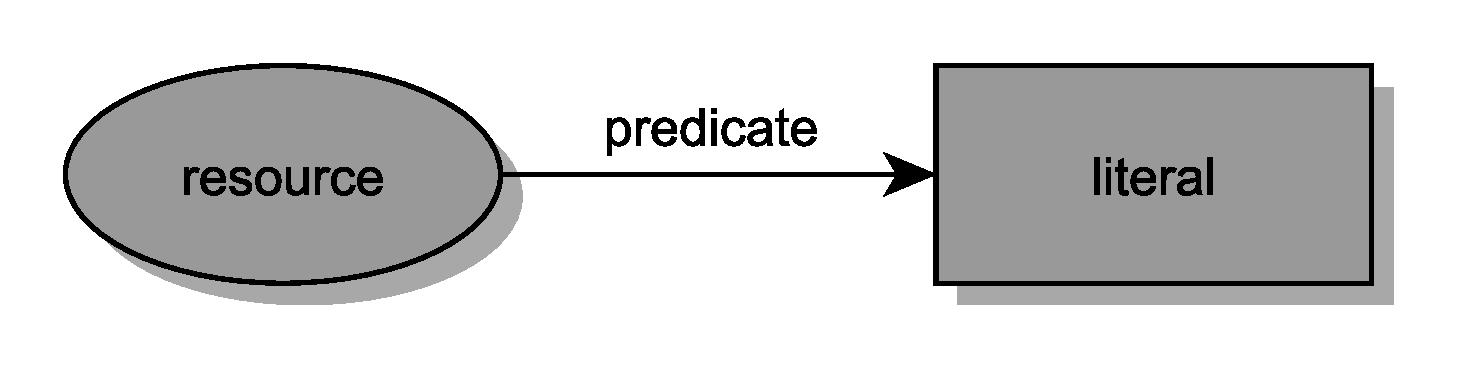
\includegraphics[
            width=0.6\textwidth,
            keepaspectratio=true,
            clip=true]
            {assets/images/rdf-triple}
        \caption{Einfacher RDF-Graph}
        \label{fig:graphisch_rdf_triple}
    \end{figure}

% paragraph graphische_darstellung (end)

\paragraph{RDF/XML} % (fold)
\label{par:rdf_xml}

RDF/XML\cite[Abschnitt 3.2]{Manola2004} ist eine verbreitete Form RDF-Dokumente zu beschreiben. Die Basis bildet hierbei die Verwendung der Extensible Markup Language (XML). In Listing \ref{lst:rdf_xml_beispiel} ist ein Beispieldokument in RDF/XML zusehen. Das in Zeile 2 zu sehende \texttt{rdf:RDF} Element zeigt, dass sich innerhalb von ihm sich die RDF-Beschreibung des Dokuments befindet. In diesem ELement werden mit \texttt{xmlns:} einige Präfixe für Namensräume  definiert, um das Dokument übersichtlicher zu halten. Alle Präfixe werden danach mit den angegebenen Namensraum ersetzt. Das \texttt{Description} in Zeile 5 stellt die Beschreibung einer Ressource im RDF-Graphen. Die URI der Ressource wird mit dem Attribut \texttt{rdf:about} definiert. Innerhalb des Description Elements befinden sich die Prädikate. In Zeile 6 steht also, dass die Ressource die Eigenschaft \texttt{exterms:enthaelt} besitzt und diese das Literal \texttt{Kekse}. Wäre das Objekt nicht wie hier ein Literal sondern eine weitere Ressource, könnte man über das Attribut \texttt{rdf:ressource} für das \texttt{exterms:enthaelt} auf diese Ressource verweisen.

\begin{lstlisting}[
    language=XML,
    caption={RDF/XML Beispiel}\label{lst:rdf_xml_beispiel},
    captionpos=t]
<?xml version="1.0"?>
<rdf:RDF xmlns:rdf="http://www.w3.org/1999/02/22-rdf-syntax-ns#"
    xmlns:exterms="http://www.example.org/terms/">

    <rdf:Description rdf:about="http://www.example.org/dose">
       <exterms:enthaelt>Kekse</exterms:enthaelt>
    </rdf:Description>
</rdf:RDF>
\end{lstlisting}
% paragraph rdf_xml (end)

\paragraph{Turtle} % (fold)
\label{par:turtle}

% paragraph turtle (end)

\begin{description}
    \item[N3] ist die Kurzform für Notation 3 und wurde von Tim Berners-Lee als Sprache für RDF entwickelt. Tripel in N3 werden dabei wie Sätze in meisten natürlichen Sprachen geschrieben. Erst das Subjekt, dann das Prädikat und am Ende das Objekt gefolgt von einen Punkt, wie in  Listing \ref{lst:n3_beispiel} zu sehen ist.
    \begin{lstlisting}[caption={Einfaches N3 Beispiel}\label{lst:n3_beispiel},captionpos=t]
<http://example.de/florian> <http://example.org/#name> "Florian" .
<http://example.de/florian> <http://example.org/#age> "28" .    \end{lstlisting} 
    Die URI \texttt{http://example.de/florian} beschreibt hierbei eine Ressource welche einen Namen \texttt{Florian} und ein Alter \texttt{28} besitzt. Es ist darauf zu achten, dass alle URI immer zwischen spitzen Klammern stehen. Da nun einzelne Prädikate recht häufig innerhalb eines Graphen auftauchen können, kann es einfach sein diese abgekürzt schreiben zu können. Hierzu ist es möglich sogenannte Präfixe (auch Namensräume genannt) am Beginn des Dokumentes zu definieren und einen so Schreibarbeit abzunehmen.

    \begin{lstlisting}[caption={Präfixe}\label{lst:n3_prefix},captionpos=t]
@prefix person: <http://example.org/#> .
<http://example.de/florian> person:name "Florian" .
<http://example.de/florian> person:age "28" .    \end{lstlisting}

    Am Anfang von Listing \ref{lst:n3_prefix} wird durch Einleiten mittels des Schlüsselwortes \texttt{@prefix} ein neuer Präfix \texttt{person:} für die URI \texttt{http://example.org/\#} festgelegt (man beachte wieder den Punkt am Ende der Zeile). Dieser Präfix kann nun überall innerhalb des Dokumentes verwendet werden, wobei die spitzen Klammern der vorherigen URI weggelassen werden können.

    \todo[inline]{Leere Knoten + kurz Turtle}
    \todo[inline]{Die englischen Fachbegriffe (also hier blank nodes oder bnodes) würde ich auch erwähnen. Das hilft dem Leser, wenn er sich englischsprachige Literatur anschaut nach dem er deine Arbeit gelesen hat.}

\end{description}

% subsubsection darstellung_von_rdf (end)

% subsection semantic_web_und_das_resource_description_framework (end)

\subsection{Ontologien} % (fold)
\label{sub:ontologien}

\subsubsection{Friend of a Friend (FOAF)} % (fold)
\label{ssub:friend_of_a_friend_}

% subsubsection friend_of_a_friend_ (end)

\subsubsection{Semantically-Interlinked Online Communities (SIOC)} % (fold)
\label{ssub:semantically_interlinked_online_communities}


Semantically-Interlinked Online Communities\footnote{\url{http://sioc-project.org/}} (SIOC, ausgesprochen \enquote{schock}) ist ein Projekt, welches von Uldis Boj\=ars und John Breslin begonnen wurde um unterschiedliche, webbasierte Diskussionslattformen(Blog, Forum, Mailinglist,\dots) untereinander verbinden zu können \cite{Breslin2005}. Der Kern von SIOC besteht aus einer Ontologie, welche den Inhalt und die Struktur diese Plattformen in ein maschinenlesbares Format bringt und es erlaubt diese auf semantischer Ebene zu verbinden. Auch soll es so möglich sein Daten von einer Plattform zu einer Anderen zu transferieren und so einfacher Inhalte austauschen zu können. Als Basis für SIOC dient RDF, die Ontologie selber wurde in RDFS und OWL designt. Um nicht das Rad neu erfinden zu müssen greift SIOC auf schon bestehende und bewährte Ontologien zurück. Für die Abbildung von Beziehungen zwischen einzelnen Personen wird Friend of a Friend\footnote{\url{http://www.foaf-project.org/}} (FOAF) und für einige Inhaltliche- und Metadaten (Titel, Inhalt, Erstelldatum, \dots) Dublin Core Terms\footnote{http://dublincore.org/documents/dcmi-terms/} eingesetzt.

\begin{figure}[ht]
    \centering
    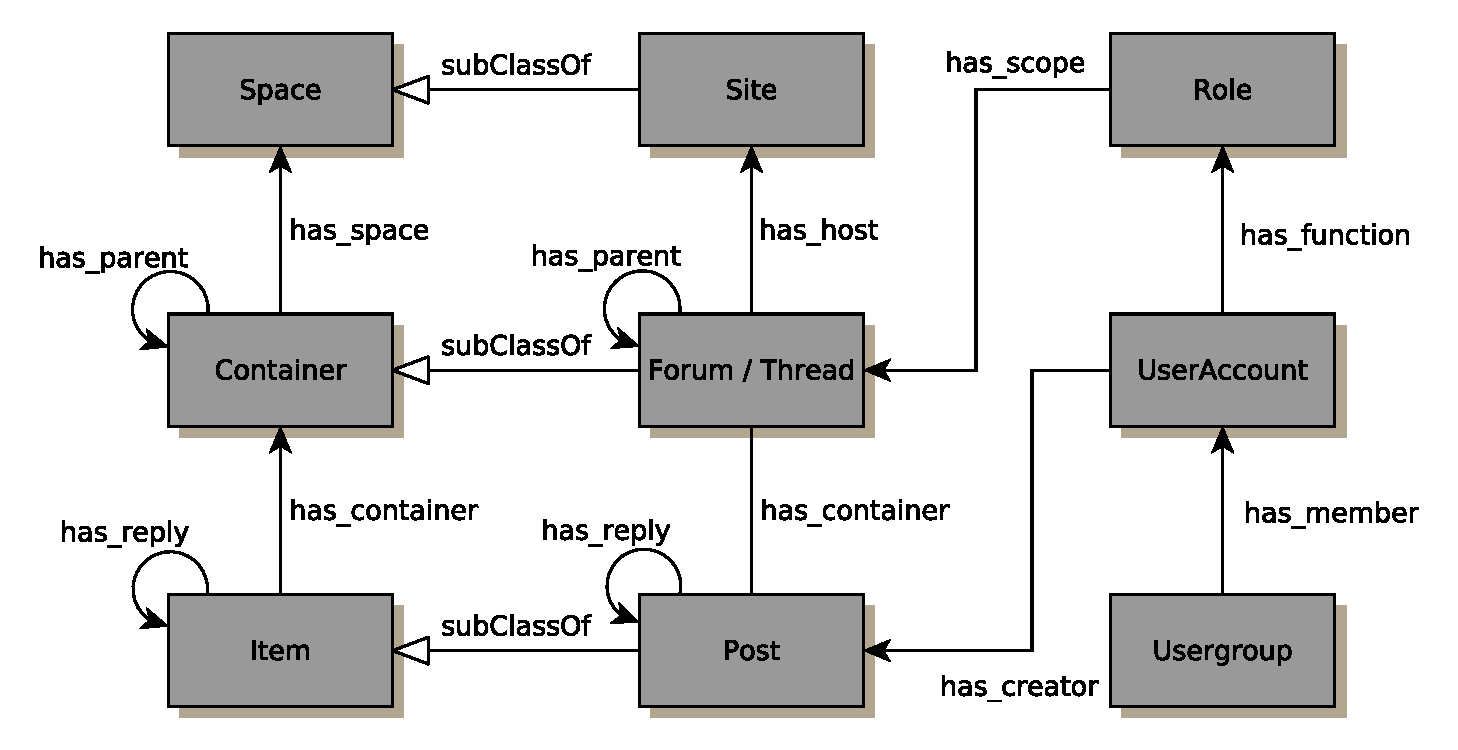
\includegraphics[
        width=\textwidth,
        keepaspectratio=true,
        clip=true]
        {assets/images/sioc_overview}
    \caption{Aufbau von SIOC (modifiziert) - Originalquelle: \cite{deri2013}}
    \label{fig:sioc_aufbau_diagramm}
\end{figure}

% subsubsection semantically_interlinked_online_communities (end)

% subsection ontologien (end)

\section{Datenverteilung} % (fold)
\label{sec:datenverteilung}

\subsection{Java Messaging Service} % (fold)
\label{sub:java_messaging_service}

% subsection java_messaging_service (end)

\subsection{Enterprise Integration Pattern und Apache Camel} % (fold)
\label{sub:enterprise_integration_pattern_und_apache_camel}

% subsection enterprise_integration_pattern_und_apache_camel (end)

% section datenverteilung (end)


\section{Lernplattformen und soziale Online-Netzwerke} % (fold)
\label{sec:lernplattformen_und_soziale_online_netzwerke}


\todo[inline]{Du könntest in dem Grundlagenkapitel auch noch auf Foren, Moodle, FB und Google+ kurz eingehen. Deren Datenmodelle und -schnittstellen können auch später erläutert werden.}

\subsection{Moodle} % (fold)
\label{sub:moodle}

Moodle\footnote{\url{https://moodle.org/}} ist ein weit verbreitetes Open Source Online LMS. Die Hauptaufgabe liegt im Verwalten von online Kursen im Bereich E-Learning. Hierzu bietet Moodle von Haus aus eine große Menge an Funktionen für die Verwaltung des Kurses und die Kommunikation zwischen Lehrenden und Lernenden. Es bietet die Möglichkeit Aufgaben die Teilnehmern zu verteilen, Fragebögen zu erstellen, zusätzlichen Kursmaterialien bereitzustellen und den Lernerfolg durch Benotung und Feedback zu kontrollieren. Funktionen für die Unterstützung des kooperativen Lernens sind ebenfalls vorhanden. Teilnehmer können Lerngruppen bilden, sich über persönliche Nachrichten austauschen, gemeinsam an Wikis arbeiten oder in Foren diskutieren. 
\begin{figure}[ht]
    \centering
    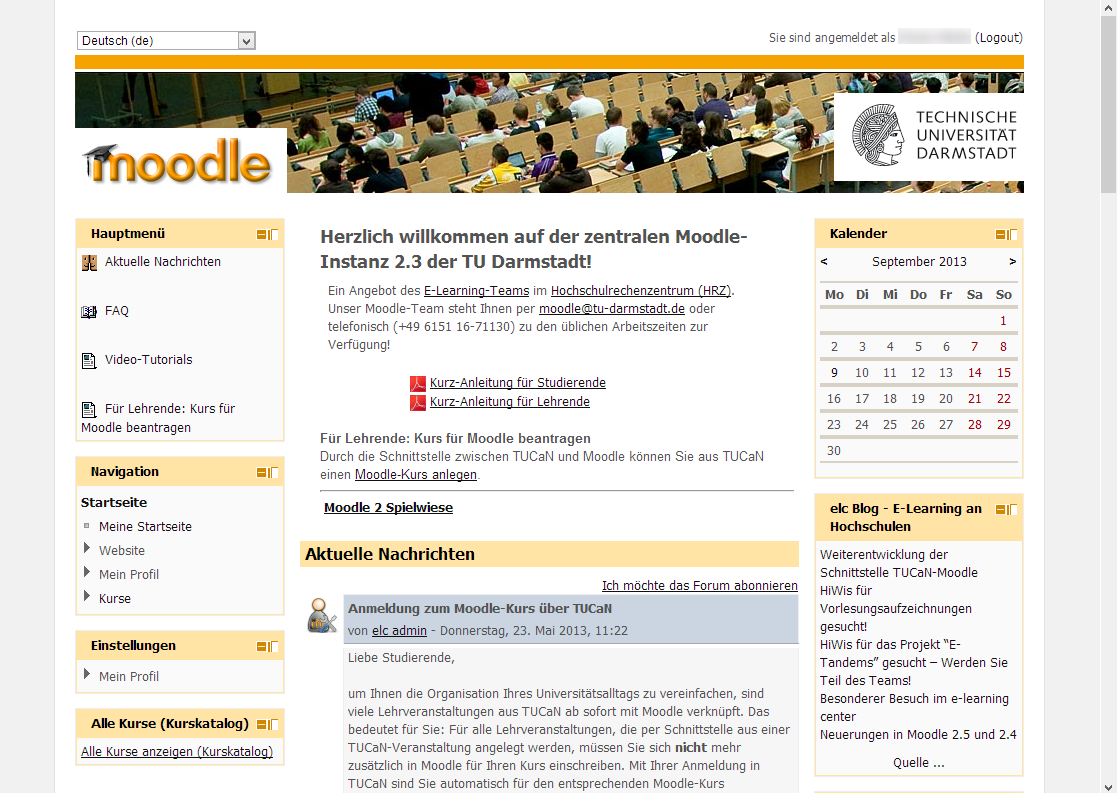
\includegraphics[
        width=0.7\textwidth,
        keepaspectratio=true,
    ]{assets/images/tud_moodle_screenshot}
    \caption{Moodle Instanz der TU Darmstadt}
    \label{fig:moodle_tud}
\end{figure}

\medskip

Moodle wurde in der Programmiersprache PHP geschrieben und unterstützt die  Datenbanken werden MySQL, PostgrSQL, MSSQL und Oracle. Die Installation von weiteren Funktionalitäten ist durch von Dritten geschriebenen Erweiterungen möglich. Seit Version 2.0 können für Moodle auch Webservices installiert werden, so können auch externe Anwendungen auf interne Funktionen und Daten zugreifen.

% subsection moodle (end)

\subsection{Canvas} % (fold)
\label{sub:canvas}

Das von der Firma Instructure\footnote{\url{https://www.instructure.com/}} entwickelte \emph{Canvas} ist ein unter Open Source Lizenz gestelltes LMS. Vom Funktionsumfang ist es Moodle nicht unähnlich. Es existiert eine Verwaltung einzelner Kurse. Innerhalb dieser Kurse können in einem Forum Diskussionen geführt und Lernmieteralien hoch- und heruntergeladenen werden. Verteilung von Aufgaben, deren Benotung und ein Benachrichtigungssystem existiert ebenfalls. Canvas erlaubt auch das Einbinden von externen Diensten zum kooperativen Lernen und Arbeiten wie Google Docs\footnote{\url{https://drive.google.com}} oder der Webkonferenz Anwendung BigBlueButton\footnote{\url{http://www.bigbluebutton.org}}.

\begin{figure}[ht]
    \centering
    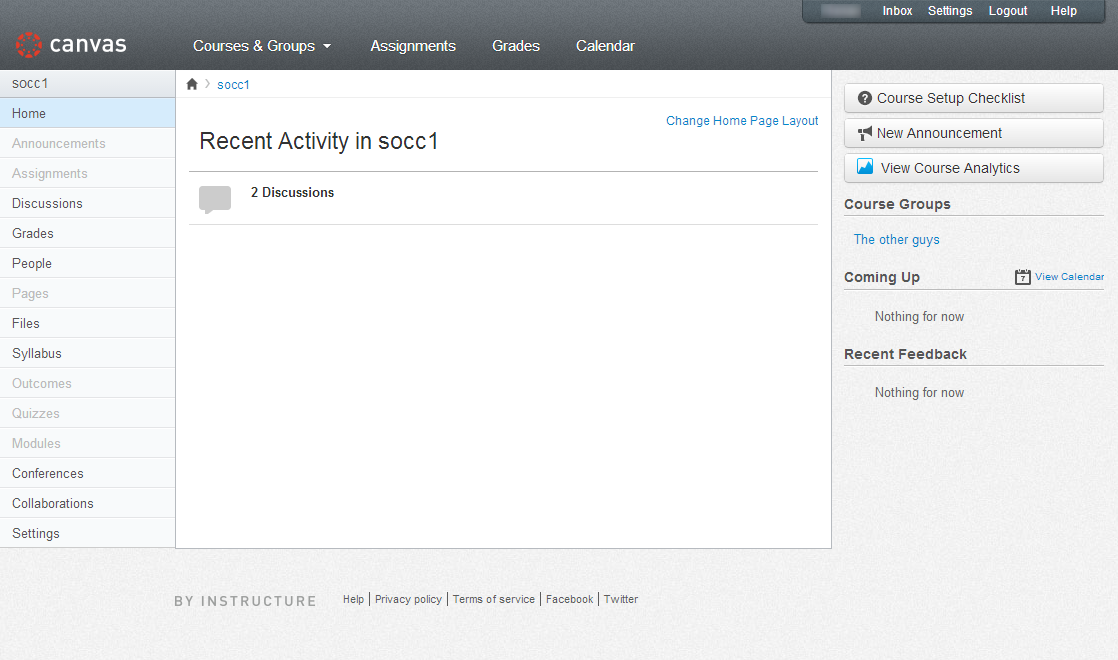
\includegraphics[
        width=0.7\textwidth,
        keepaspectratio=true,
    ]{assets/images/canvas_lms}
    \caption{Instructure Canvas}
    \label{fig:canvas_lms}
\end{figure}

Canvas wird mittels des Webframeworks \emph{Ruby on Rails}\footnote{http://rubyonrails.org/} entwickelt. Das Aussehen ist etwas moderner, als das von Moodle und es wird sehr stark auf die neuesten Webtechnologien wie HTML5 CSS3 und JQuery gesetzt. Eine Erweiterung der Funktionalität von Canvas ist durch das einbinden von Programmen möglich, die den \emph{Learning Tools Interoperability™} (LTI) Standard erfüllen. Einige solcher Programme finden sich auf der Webseite \url{https://www.edu-apps.org}. Unter anderem Programme zum Suchen und Einbinden von Youtube Videos, Wikipedia Artikeln, GitHub Gists\footnote{\url{https://gist.github.com}} und vielen weiteren.

% subsection canvas (end)

\subsection{Youtube} % (fold)
\label{sub:youtube}

Die Youtube\footnote{\url{https://www.youtube.com}} Webseite gehört wohl heute zu den beliebtesten Anlaufpunkten im Internet, wenn es um das Thema Videos geht. Monatlich nutzen über 1 Milliarde Nutzer die Seite und pro Minute werden 100 Stunden neuer Videos hochgeladen \cite{youtube2013statistics}. Doch nicht das komplette Videomaterial besteht aus Katzen, Musik oder Videos von Unfällen. Ein Teil der Benutzer die eigene Videos hochladen, wollen anderen Dinge beibringen, weil es sie schon immer interessierte oder früher selber Probleme damit hatten. Einer erklärt die Logarithmengesetze, ein anderer wie man Feuer ohne Feuerzeug macht und eine ganz andere gibt Schönheitstipps. Youtube ist also auch im E-Learning Bereich gut einsetzbar. Lehrende können eigene Videos hochladen, von anderen interessante Videos in Playlisten zusammenfassen und die Lernenden können über Kommentare Fragen zum Inhalt stellen. 

% subsection youtube (end)

\subsection{Facebook} % (fold)
\label{sub:facebook}

Das soziale Online-Netzwerk Facebook\footnote{\url{https://www.facebook.com/}} kann mit rund 699 Millionen aktiven Benutzern täglich \cite{Facebook2013} zu den aktuell beliebtesten Vertretern seiner Art bezeichnet werden. Facebook erlaubt es, wie alle sozialen Online-Netzwerke, bekannte Personen in Freundeslisten zusammen zufassen und mit ihnen private Nachrichten auszutauschen. Beiträge wie Texte, Fotos oder Videos können auf einer Art Pinnwand der \enquote{Wall} öffentlich oder nur mit Freunden geteilt werden. Benutzer mit gemeinsamen Interessen können dazu eigene Gruppen bilden und dort auf einer eigen Wall Beiträge veröffentlichen oder die anderer kommentieren. Wie in der Einleitung schon erklärt zeigt Qiyun Wang et. al. \cite{Wang2012} das sich Facebook, wenn auch mit Einschränkungen wunderbar zur Verwaltung und Nutzung durch Lernkurse und Lerngruppen eignet. 


% subsection facebook (end)

\subsection{Google+} % (fold)
\label{sub:google_plus}

Google+\footnote{https://plus.google.com} ist ein 2011 von Google gestartetes soziales Online-Netzwerk. Seit Anfang 2013 ist Google+, von der Anzahl der aktiven Benutzer her gesehen, auf Platz 2 hinter Marktführer Facebook \cite{Thomas2013}. Vom Funktionsumfang sind sich beide sehr ähnlich. Auf Google+ können andere Benutzer in sogenannten \enquote{Circles} sortiert werden. Dies entspricht ungefähr den auf Facebook genutzten Freundeslisten. Jeder Benutzer hat einen eigenen \enquote{Stream} in dem er Beiträge öffentlich oder nur für ein oder mehrere Circles verfassen kann. Das Gründen von Gruppen für bestimmte Interessensbereiche ist auch in Google+ möglich und werden dort als \enquote{Communities} bezeichnet. Eines der interessantesten Funktionen von Google+ dürfte die Einführung von \enquote{Google Hangout} sein. Hier können Benutzer neben Chats auch Videokonferenzen mit bis zu zehn anderen abhalten, ohne einen externen Service wie Skype\footnote{\url{http://www.skype.com/}} zu nutzen. Diese Funktion wäre gut für den Einsatz in E-Learning nutzbar. Ein Tutor könnte so in kleiner Runde Fragestunden abhalten oder Gruppen Treffen abhalten.

% subsection google_ (end)

% section lernplattformen_und_soziale_online_netzwerke (end)

\section{Verwandte Arbeiten und Projekte} % (fold)
\label{sec:verwandte_arbeiten_und_projekte}


\subsection{What happens when Facebook is gone?} % (fold)
\label{sub:what_happens_when_facebook_is_gone}

Frank McCown und Michael L. Nelson beschreiben in ihrem Bericht \enquote{What happens when Facebook is gone?}\cite{McCown2009}, wie Möglichkeiten aussehen können, die unsere Daten von sozialen Online-Netzwerken (hier im speziellen Fall von Facebook) für uns und die Nachwelt archivieren können. Zum Beispiel, wenn eine Person einen großen Teil seines persönlichen Lebens auf Facebook verbringt und plötzlich stirbt. Wie sollen seine Angehörigen an nicht öffentliche Texte, Bilder, Videos heran kommen, wenn sie in der Regel keinen Zugriff auf das Benutzerkonto haben, da der Verstorbene so etwas nicht vorhersehen konnte. Oder wenn ein Benutzer mit seinen Daten in ein anderes soziales Online-Netzwerk umziehen will, sei dies bei Facebook zum damaligen Zeitpunkt nur schwer möglich.

\begin{quote}
    \enquote{It is also likely he was not prepared to die at such a young age, and much of his personal life, which lies in the digital \grqq cloud\grqq, may never be accessible to his loved ones}
    \cite[S.\,251]{McCown2009}
\end{quote}

Zum Anlegen eines solchen Archivs wurden mehrere Ansätze vorgestellt. Die einfachste Ansatz wäre die E-Mail-Benachrichtigung zu aktivieren und alle neuen Beiträge in einem E-Mail-Postfach zu sichern. So können aber nur neuen alle Beiträge erfasst werden, alte bleiben weiterhin in Facebook. Eine sehr aufwändige Möglichkeit wäre es Bildschirmfotos von den Beiträgen zu machen und diese durch ein Texterkennungsprogramm laufen zu lassen. Die dadurch erzeugten Dateien können dann in einer Datenbank gespeichert werden. Heutige Internetbrowser zusätzlich zum Anzeigen von Webseite auch der Herunterladen selbiger an. Dabei wird die HTML-Datei inklusive aller darin enthaltenen weiteren Dateien wie Bilder, Videos und CSS-Dateien gespeichert. Die so archivierte Seite hat dann im beschränkten Umfang genau das gleiche Aussehen und Verhalten wie die original Seite. Ebenfalls wäre eine Nutzung der von Facebook bereitgestellten API für Anwendungen eine Überlegung wert. 2009 war diese API noch sehr eingeschränkt. Gerade der Zugriff auf Beiträge und private Nachrichten war nicht möglich \cite[S.\,253, Table 1]{McCown2009}. Für die Implementierung eines Beispiel Programms wurde ein fünfter Ansatz gewählt. Über einen sogenannten Webcrawler oder eine Erweiterung für den Browser werden relevante Seiten automatisch heruntergeladen und in einen Archiv abgelegt. Dynamische Inhalte sollen kein Problem darstellen, da Seite erst heruntergeladen wird, wenn alle Aufrufe dynamischer Funktionen abgeschlossen ist. Die archivierten Dateien können dann mittels Datamining Techniken verarbeitet und als Atom/RSS Feed\footnote{\url{http://www.rssboard.org/rss-specification}} bereitgestellt werden. 

% subsection what_happens_when_facebook_is_gone_ (end)

\subsection{Reclaim Social} % (fold)
\label{sub:reclaim_social}

Hat sich nicht jeder schon einmal vor den Rechner gesessen um, zum Beispiel, nach einen Bild gesucht das man irgendwann auf irgendeinem der unzähligen sozialen Netzwerke hochgeladen hat, einem aber partout nicht einfallen will wo? Wann und wo habe habe ich den Beitrag geschrieben, der perfekt zu meiner aktuellen Arbeit passen würde? Solche oder ähnliche Fragen wurden sicherlich schon mehrere Millionen mal von verschiedenen Menschen in der Welt des Internets gestellt. Wer hätte in so einen Fall nicht gerne alles was man über die letzten Jahre an verschiedenen Stellen im Netz geschrieben, hochgeladen oder als für ihn wichtig markiert hat zentral gespeichert um es durchsuchen zu können? Genau diesem Thema haben sich Sascha Lobo und Felix Schwenzel angenommen und auf der Netzkonferenz re:publica\footnote{\url{http://re-publica.de/}} 2013 ihr gestartetes Projekt \enquote{Reclaim Social} \cite{Schwenzel2013} vorgestellt.

\todo[inline]{Das klingt ein wenig wie ein Werbetext ;-)}

\medskip

Ziel mit diesem Projektes soziale Medien aus allen möglichen Quellen auf seinen eigenen Blog zu spiegeln und so einen zentrale Anlaufstelle für seine eigenen Inhalte schaffen. Aufbauend auf der weit verbreiteten Blogsoftware \enquote{WordPress\footnote{\url{http://wordpress.org/}}} und der dafür vorhandenen Erweiterung \enquote{FeedWordPress}\footnote{\url{http://feedwordpress.radgeek.com/}}. Diese Kombination ermöglichst alle Internetseiten, welche einen RSS Feed anbieten, in die Datenbank von WordPress zu spiegeln. Das Problem hierbei besteht darin, dass einige sehr beliebte Internetseiten solche RSS Feeds nicht anbieten (Facebook, Google+) oder eingestellt haben (\url{https://twitter.com}). Für einige solcher Seiten wurden \enquote{proxy-scripte}\cite[Tech Specs Details]{Schwenzel2013} implementiert, welche für diese einen RSS Feed emulieren. Zugleich können in den Feeds enthaltende Medien, wie Bilder und Videos(bisher nur als Referenz), heruntergeladen und in WordPress gespeichert werden. So ist es möglich alle gespiegelten Daten einfach zu durchsuchen oder nach bestimmten Kriterien zu filtern. Zusätzlich können alle Freunde, welche auch Reclaim Social einsetzen, in einen Kontaktliste eingetragen und so auch deren Inhalte eingebunden werden.

\medskip

Aktuell befindet sich dieses Projekt noch im Alpha Stadium und die Installation ist relativ kompliziert. Es ist aber geplant eine eigene Erweiterung für WordPress zu schreiben \enquote{he goal is to build just one Reclaim Social-plugin for any wordpress user}\cite[How Does It Work]{Schwenzel2013}

% subsection reclaim_social (end)

% section verwandte_arbeiten_und_projekte (end)

% chapter grundlagen (end)